\documentclass[hidelinks,12pt,dvipsnames,border=2pt]{standalone}
%\usepackage[top=0.7in, bottom=0.8in, left=1in, right=1in]{geometry}
\usepackage{tikz}
\usepackage{hyperref}
\usetikzlibrary{arrows}
\usetikzlibrary{shapes}
\usepackage{enumitem}
\usepackage{bm}
\usepackage{mathdots}
\usepackage{amsmath}
\usepackage{tcolorbox}
\usetikzlibrary{shadings}
\usetikzlibrary{decorations.pathreplacing}
\usepackage{helvet}
\usepackage{url}
\usepackage{graphicx}
\usetikzlibrary{arrows.meta,positioning,fit,calc}
\renewcommand{\familydefault}{\sfdefault}


\usetikzlibrary{arrows,decorations.pathmorphing,backgrounds,fit,positioning,shapes.symbols,chains}

\begin{document}
	
% trim=left botm right top
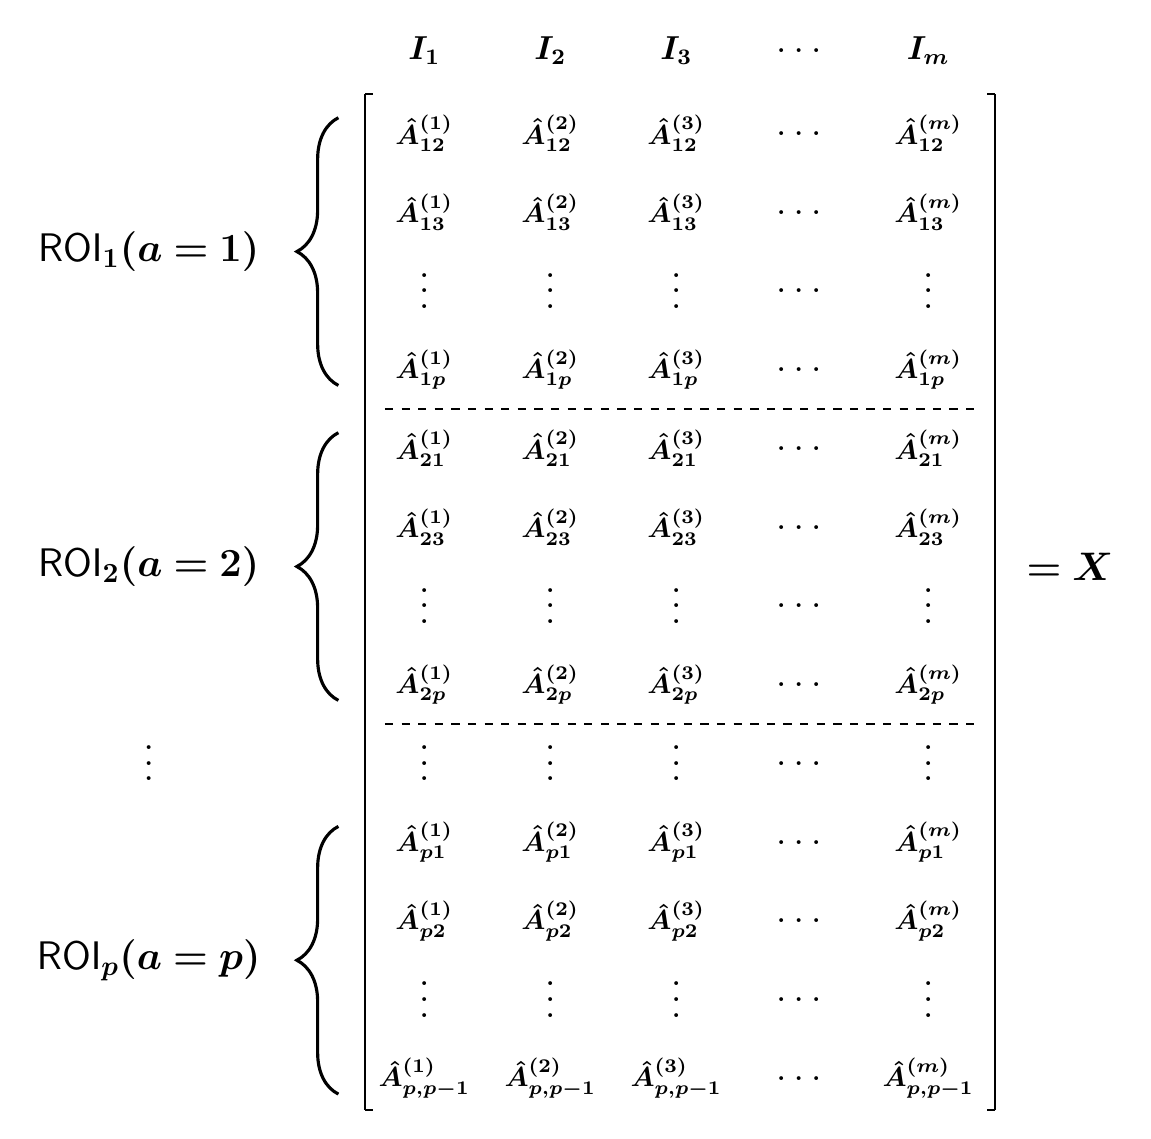
\begin{tikzpicture}
\node at (0,-0.45) {\large \bm{$I_1$}};
\node at (1.6,-0.45) {\large \bm{$I_2$}};
\node at (3.2,-0.45) {\large \bm{$I_3$}};
%\node at (4.8,-0.45) {\large \bm{$I_4$}};
\node at (4.8,-0.45) {\Large $\dots$};
\node at (6.4,-0.45) {\large \bm{$I_m$}};

%\draw [decorate,decoration={brace,amplitude=25pt,aspect=0.5},xshift=-4pt,yshift=0pt,line width=0.4mm,draw=cyan] (-0.25,0) -- (8.5,0) node [black,xshift=9pt] {\footnotesize};
%\node at (4,1.35) {\Large Instances};

\draw [decorate,decoration={brace,amplitude=15pt,aspect=0.5,mirror},xshift=-4pt,yshift=0pt,line width=0.4mm,draw=black] (-0.95,-1.3) -- (-0.95,-4.7) node [black,xshift=9pt] {\footnotesize};
\node at (-3.5,-3) {\Large \bm{$\text{ROI}_1 (a=1)$}};

\draw [decorate,decoration={brace,amplitude=15pt,aspect=0.5,mirror},xshift=-4pt,yshift=0pt,line width=0.4mm,draw=black] (-0.95,-5.3) -- (-0.95,-8.7) node [black,xshift=9pt] {\footnotesize};
\node at (-3.5,-7) {\Large \bm{$\text{ROI}_2 (a=2)$}};

\draw [decorate,decoration={brace,amplitude=15pt,aspect=0.5,mirror},xshift=-4pt,yshift=0pt,line width=0.4mm,draw=black] (-0.95,-10.3) -- (-0.95,-13.7) node [black,xshift=9pt] {\footnotesize};
\node at (-3.5,-12) {\Large \bm{$\text{ROI}_p (a=p)$}};

\node at (-3.5,-9.35) {\Large \textbf{$\vdots$}};

% row 1
\node at (0,-1.5) {\bm{$\hat{A}^{(1)}_{12}$}};
\node at (1.6,-1.5) {\bm{$\hat{A}^{(2)}_{12}$}};
\node at (3.2,-1.5) {\bm{$\hat{A}^{(3)}_{12}$}};
%\node at (4.8,-1.5) {\bm{$\hat{A}^{(4)}_{12}$}};
\node at (4.8,-1.5) {\Large \textbf{$\dots$}};
\node at (6.4,-1.5) {\bm{$\hat{A}^{(m)}_{12}$}};

% row 2
\node at (0,-2.5) {\bm{$\hat{A}^{(1)}_{13}$}};
\node at (1.6,-2.5) {\bm{$\hat{A}^{(2)}_{13}$}};
\node at (3.2,-2.5) {\bm{$\hat{A}^{(3)}_{13}$}};
%\node at (4.8,-2.5) {\bm{$\hat{A}^{(4)}_{13}$}};
\node at (4.8,-2.5) {\Large $\dots$};
\node at (6.4,-2.5) {\bm{$\hat{A}^{(m)}_{13}$}};

% row 3
\node at (0,-3.35) {\Large \textbf{$\vdots$}};
\node at (1.6,-3.35) {\Large \textbf{$\vdots$}};
\node at (3.2,-3.35) {\Large \textbf{$\vdots$}};
%\node at (4.8,-3.35) {\Large \textbf{$\vdots$}};
\node at (4.8,-3.5) {\Large \textbf{$\dots$}};
\node at (6.4,-3.35) {\Large \textbf{$\vdots$}};

% row 4
\node at (0,-4.5) {\bm{$\hat{A}^{(1)}_{1p}$}};
\node at (1.6,-4.5) {\bm{$\hat{A}^{(2)}_{1p}$}};
\node at (3.2,-4.5) {\bm{$\hat{A}^{(3)}_{1p}$}};
%\node at (4.8,-4.5) {\bm{$\hat{A}^{(4)}_{1p}$}};
\node at (4.8,-4.5) {\Large \textbf{$\dots$}};
\node at (6.4,-4.5) {\bm{$\hat{A}^{(m)}_{1p}$}};

\draw[line width=0.3mm,dashed] (-0.5,-5) -- (7,-5);

% row 5
\node at (0,-5.5) {\bm{$\hat{A}^{(1)}_{21}$}};
\node at (1.6,-5.5) {\bm{$\hat{A}^{(2)}_{21}$}};
\node at (3.2,-5.5) {\bm{$\hat{A}^{(3)}_{21}$}};
%\node at (4.8,-5.5) {\bm{$\hat{A}^{(4)}_{21}$}};
\node at (4.8,-5.5) {\Large \textbf{$\dots$}};
\node at (6.4,-5.5) {\bm{$\hat{A}^{(m)}_{21}$}};

% row 6
\node at (0,-6.5) {\bm{$\hat{A}^{(1)}_{23}$}};
\node at (1.6,-6.5) {\bm{$\hat{A}^{(2)}_{23}$}};
\node at (3.2,-6.5) {\bm{$\hat{A}^{(3)}_{23}$}};
%\node at (4.8,-6.5) {\bm{$\hat{A}^{(4)}_{23}$}};
\node at (4.8,-6.5) {\Large \textbf{$\dots$}};
\node at (6.4,-6.5) {\bm{$\hat{A}^{(m)}_{23}$}};

% row dots
\node at (0,-7.35) {\Large \textbf{$\vdots$}};
\node at (1.6,-7.35) {\Large \textbf{$\vdots$}};
\node at (3.2,-7.35) {\Large \textbf{$\vdots$}};
%\node at (4.8,-7.35) {\Large \textbf{$\vdots$}};
\node at (4.8,-7.5) {\Large \textbf{$\dots$}};
\node at (6.4,-7.35) {\Large \textbf{$\vdots$}};

% row dots
\node at (0,-8.5) {\bm{$\hat{A}^{(1)}_{2p}$}};
\node at (1.6,-8.5) {\bm{$\hat{A}^{(2)}_{2p}$}};
\node at (3.2,-8.5) {\bm{$\hat{A}^{(3)}_{2p}$}};
%\node at (4.8,-8.5) {\bm{$\hat{A}^{(4)}_{2p}$}};
\node at (4.8,-8.5) {\Large \textbf{$\dots$}};
\node at (6.4,-8.5) {\bm{$\hat{A}^{(m)}_{2p}$}};

\draw[line width=0.3mm,dashed] (-0.5,-9) -- (7,-9);

\node at (0,-9.35) {\Large \textbf{$\vdots$}};
\node at (1.6,-9.35) {\Large \textbf{$\vdots$}};
\node at (3.2,-9.35) {\Large \textbf{$\vdots$}};
%\node at (4.8,-9.35) {\Large \textbf{$\vdots$}};
\node at (4.8,-9.5) {\Large \textbf{$\dots$}};
\node at (6.4,-9.35) {\Large \textbf{$\vdots$}};

\node at (0,-10.5) {\bm{$\hat{A}^{(1)}_{p1}$}};
\node at (1.6,-10.5) {\bm{$\hat{A}^{(2)}_{p1}$}};
\node at (3.2,-10.5) {\bm{$\hat{A}^{(3)}_{p1}$}};
%\node at (4.8,-10.5) {\bm{$\hat{A}^{(4)}_{p1}$}};
\node at (4.8,-10.5) {\Large \textbf{$\dots$}};
\node at (6.4,-10.5) {\bm{$\hat{A}^{(m)}_{p1}$}};

\node at (0,-11.5) {\bm{$\hat{A}^{(1)}_{p2}$}};
\node at (1.6,-11.5) {\bm{$\hat{A}^{(2)}_{p2}$}};
\node at (3.2,-11.5) {\bm{$\hat{A}^{(3)}_{p2}$}};
%\node at (4.8,-11.5) {\bm{$\hat{A}^{(4)}_{p2}$}};
\node at (4.8,-11.5) {\Large \textbf{$\dots$}};
\node at (6.4,-11.5) {\bm{$\hat{A}^{(m)}_{p2}$}};

\node at (0,-12.35) {\Large \textbf{$\vdots$}};
\node at (1.6,-12.35) {\Large \textbf{$\vdots$}};
\node at (3.2,-12.35) {\Large \textbf{$\vdots$}};
%\node at (4.8,-12.35) {\Large \textbf{$\vdots$}};
\node at (4.8,-12.5) {\Large \textbf{$\dots$}};
\node at (6.4,-12.35) {\Large \textbf{$\vdots$}};

\node at (0,-13.5) {\bm{$\hat{A}^{(1)}_{p,p-1}$}};
\node at (1.6,-13.5) {\bm{$\hat{A}^{(2)}_{p,p-1}$}};
\node at (3.2,-13.5) {\bm{$\hat{A}^{(3)}_{p,p-1}$}};
%\node at (4.8,-13.5) {\bm{$\hat{A}^{(4)}_{p,p-1}$}};
\node at (4.8,-13.5) {\Large \textbf{$\dots$}};
\node at (6.4,-13.5) {\bm{$\hat{A}^{(m)}_{p,p-1}$}};

\draw[line width=0.3mm] (-0.75,-13.9) -- (-0.75,-1);
\draw[line width=0.3mm] (-0.75,-1) -- (-0.65,-1);
\draw[line width=0.3mm] (-0.75,-13.9) -- (-0.65,-13.9);

\draw[line width=0.3mm] (7.25,-13.9) -- (7.25,-1);
\draw[line width=0.3mm] (7.25,-1) -- (7.15,-1);
\draw[line width=0.3mm] (7.25,-13.9) -- (7.15,-13.9);

\node at (8.2,-7) {\Large \bm{$= X$}};
\end{tikzpicture}

\end{document}